\documentclass{vldb}
\usepackage{graphicx}
\usepackage{float}
\usepackage{hyperref}
\usepackage[colorinlistoftodos]{todonotes}
\usepackage[title]{appendix}
\usepackage{listings}
\usepackage{color}
\usepackage{balance}



\title{Assignment 1}
\author{
	Wojciech Sidor\\
	number\\
	Vrije Universiteit Amsterdam\\
	@student.vu.nl
	\and
	Andrei Tatar\\
	number\\
	Vrije Universiteit Amsterdam\\
	@student.vu.nl
	\and
	Alessandro Zonta\\
	2562464\\
	Vrije Universiteit Amsterdam\\
	ama228@student.vu.nl
}
\date{\today}

\begin{document}
\maketitle

\section{Introduction}

	
\section{Task 1: Explore a small data set}
	RapidMiner?!?!?!?
	
	\subsection{Exploration}
	In the data sets there are 104 records.
	Most of them are bachelor or economics students.
	In third position, there are Artificial Intelligence students.
	In Appendix \ref{program} are visible all the different programs of study.
	The first five attributes can be seen like Boolean attributes because there are only yes or no answer.
	This is true although in the data every attribute has a different range.
	For example column two has yes/no, column three has 0/1 and so on.
	With the fifth attribute, we can find more possibility: there are five choices and a lot of different format of representation.
	In Appendix \ref{chocolate} is visible this fact.
	The majority of the people think that chocolate does not make people fat or slim but a lot of people think that chocolate make people fat.
	There were no standard to respect so everyone chose the own standard.
	In the data is possible to find a lot different representations like day-month, day/month/year or day-month-year.
	There are also different standards to represent month that has only one number, like March.
	Someone wrote only the number 3 and other people wrote 03.
	Notice that we are sure that two people have the same birthday and the same age (both were born in 1991) and there are another four people with the same birthday.
	Our class respect the birthday paradox (Figure \ref{fig1}).
	\begin{figure}[h]
		\centering
		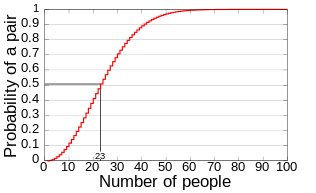
\includegraphics[scale=0.5]{0.png}
		\caption{Birthday Paradox}
		\label{fig1}
	\end{figure}

	Apparently one value in stress row is malformed because the input range had to be 0-100 but someone wrote 39087.
	I think for a correct use of this data, that value should be correct.
	In Appendix \ref{money} is visible the graphic related to how much money we think we can obtain.
	The majority of the people think we can earn only 1£. 
	Is funny that the common thing that people want to have a good day is have a good weather outside, in particular the presence of the sun.
	This means that a lot of people haven't a good day because in Amsterdam is very common have a cloudy day. The word distribution is visible in Appendix \ref{word}.
		
	\subsection{Basic classification/regression}
	
\section{Task 2: Compete in a Kaggle Competition to Predict Titanic Surviv}

	\subsection{Preparation}
	\subsection{Classification and Evaluation}

\section{Task 3: Research and theory}

	\subsection{Research: State of the art solutions}
	The competition chose for this evaluation is the \textbf{Flight quest phase 1} \cite{first}.
	The airlines are constantly looking for ways to make flights more efficient.
	From gate conflicts to operational challenges to air traffic management, the dynamics of a flight can change quickly and lead to costly delays.
	Advancements in real-time big data analysis are changing the course of flight as we all know it.
	Imagine if the pilot could augment their decision-making process with ``real time business intelligence'', some kind of information available in the cockpit that would allow them to adjust their flight plans.
	The goal of this challenge is use the different data sets found on the challenge page to develop a usable and scalable algorithm that delivers a real-time fight profile to the pilot, helping them make flight more efficient.

	The competition started in November 2012 and ended in March 2013. 173 teams joined the competition, with in total 236 players. All the teams made 3067 submission during the challenge. The first prize were \$100.000, the second \$50.000 and teams earn money until fifth place.

	The data used for the competition was split into five data sets released over the course of the competition.
	The first two data sets released contains all the flight and the weather information for domestic US flights during the corresponding days.
	The last data sets had this information for each day up to a predetermined cutoff time.
	FlightStats, Inc. and other sources provided data.
	The model must be structured so that it makes each test day's final test data set predictions based on no information in the final evaluation test data other than the information from that day, which will be in an appropriately named folder.
	The relevant data is divided into folders by day.
	For these purposes, a "day" includes all of the time from 1amPST/4amEST/9amUTC on that day until the same time on the next day.
	So Nov. 11, 2012 is considered to be from 9am UTC on Nov. 11, 2012 until 9am UTC on Nov. 12, 2012.

	The teams are predicting both the runway arrival time and the gate arrival time, so they have two predictions for each airplane.
	Their predictions were evaluated using the root mean squared error (RMSE) between the predicteds and the truth:
		$$RMSE=\sqrt{\frac{1}{n}\sum_{i=1}^n \left | y_i - \hat{y}_i \right |} $$
	They separately compute also the RMSE for gate arrival times and runway arrival times, and use a weighted average of the two:
		$$RMSE_Final=(0.75×RMSE_Gate)+(0.25×RMSE_Runway)$$
	The Team \textit{Gxav \&*} won the competition.
	Xavier Conort, Cao Hong, Clifton Phua, Ghim-Eng Yap and Kenny Chua from Singapore formed the team.
	They used a mixture of gradient boosting and random forest models to predict gate and runway arrivals time.
	Their success derived from careful feature selection.
	Their final model use only 58 and 84 features for gate and runway arrivals from the total 258 features.
	They spent most of their efforts in feature engineering because the algorithm they used are very standard for Kagglers.
	Their final feature selection is a collection of flight statistics and attributes, weather information during the flights, traffic in airports and weather conditions at arrival.
	They were also very careful to discard features likely to expose them to the risk of over-fitting their model. 
	They spent a tremendous time exploring the numerous datasets, visualizing the data, understanding which data could bring value, and elaborating a strategy to convert all this data in usable features before producing their first model. 
	The most challenging part of the data quest was the timeline of the competition. 
	The most critical deadline was just a few days after Chinese New Year.
	Chinese New Year is a 4-day period during which you are supposed to spend time with your family, not with data and algorithms!

	The second group classified (Team \textit{As High As Honor}) used a two-step approach that combined the results of a generalized linear model that encoded intuition about important variables with refinements derived from a random forest model.
	The third group classified (Team \textit{Taki}) used a six layer model based on successive ridge regressions and gradient boosting machines to model both gate and runway arrival times.
	This approach used only 56 features extracted from the raw data.
		
	
	
	\subsection{Theory: MSE verse MAE}
	The MSE of an estimator $\hat{\theta}$ with respect to the unknown parameter $\theta$ is defined as\\ $MSE(\hat{\theta})=E[(\hat{\theta}-\theta)^2]$
		
	The mean absolute error is given by\\ $MAE=\frac{1}{n}\sum_{i=1}^n \left | f_i - y_i \right | = \frac{1}{n}\sum_{i=1}^n \left | e_i \right |$
	\subsection{Theory: Analyze a less obvious data set}
	
\begin{thebibliography}{99}

	\bibitem{first}{Kaggle quest at \textit{\href{http://www.gequest.com/c/flight}{http://www.gequest.com/c/flight}}}
	
	
	
\end{thebibliography}	
		
\begin{appendices}
\onecolumn
\section{Program Distribution}\label{program}
		\begin{figure}[h]
			\centering
			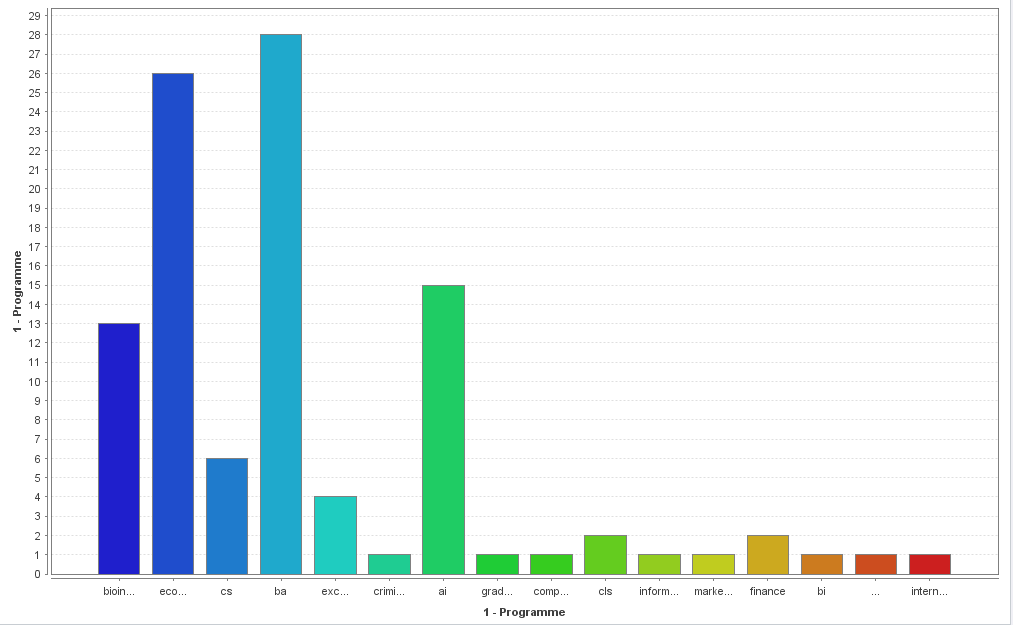
\includegraphics[scale=0.4]{1.png}
			\caption{Program}
			\label{fig2}
		\end{figure}
\section{Chocolate Distribution}\label{chocolate}
		\begin{figure}[h]
			\centering
			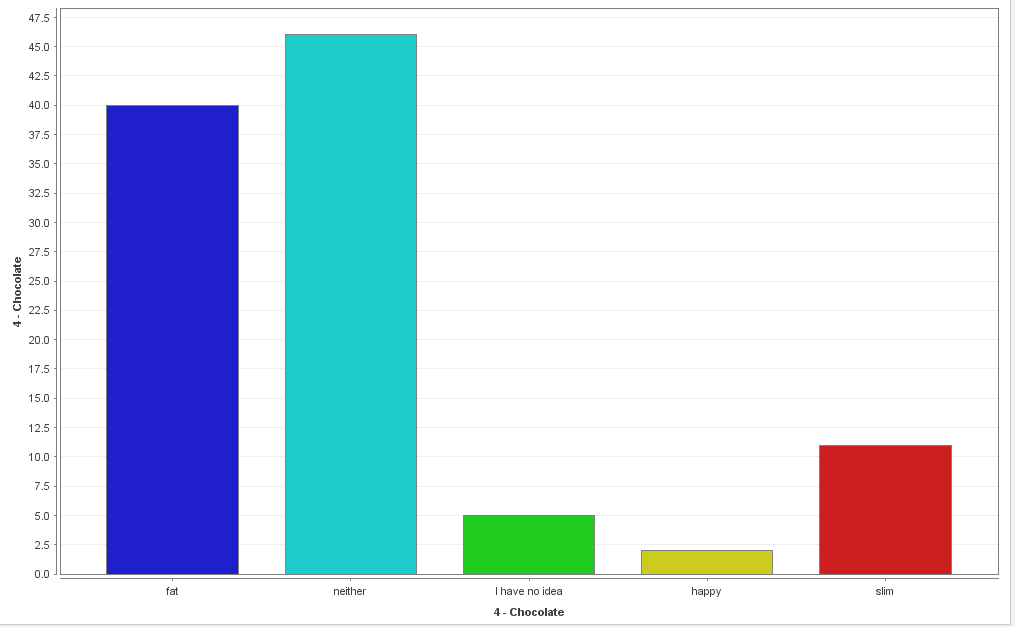
\includegraphics[scale=0.4]{2.png}
			\caption{Chocolate Distribution}
			\label{fig3}
		\end{figure}
\section{Money Distribution}\label{money}
		\begin{figure}[h]
			\centering
			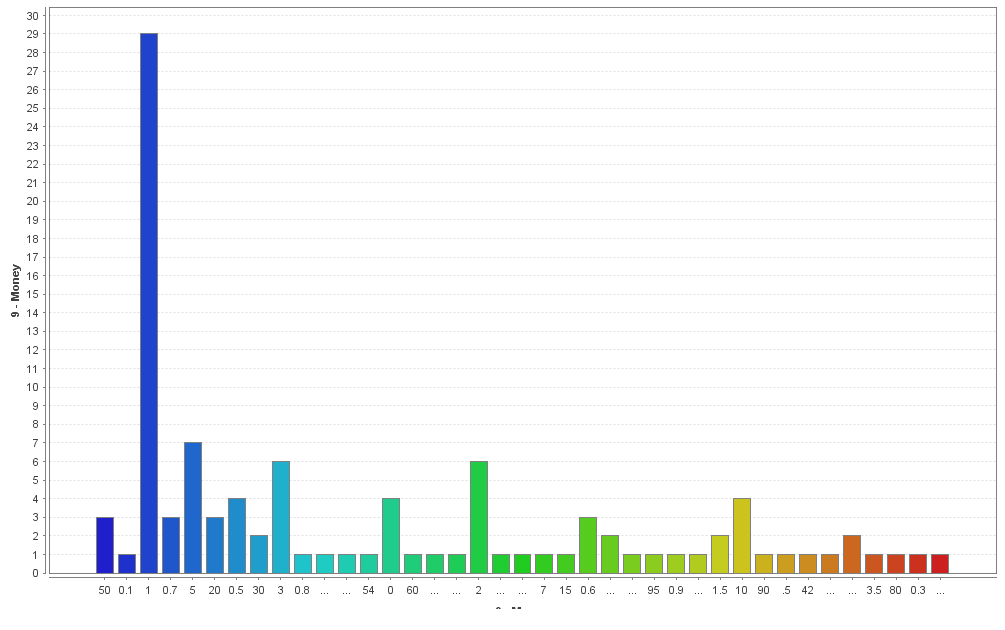
\includegraphics[scale=0.4]{3.png}
			\caption{Money distribution}
			\label{fig4}
		\end{figure}
\section{Words}\label{word}
		\begin{figure}[h]
			\centering
			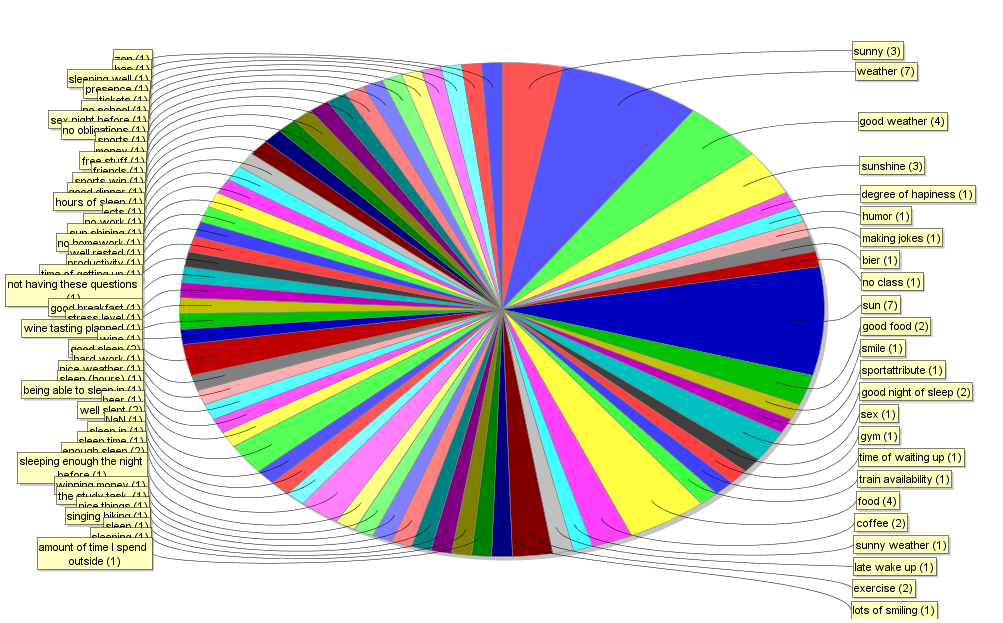
\includegraphics[scale=0.5]{5.png}
			\caption{Have a good day words 1}
			\label{fig6}
		\end{figure}
		\begin{figure}[h]
			\centering
			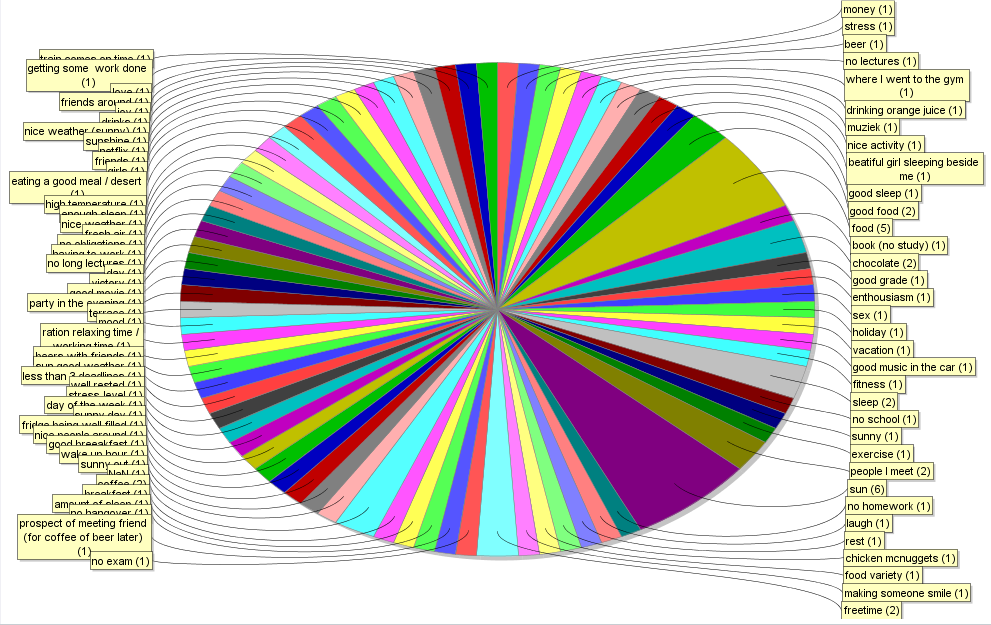
\includegraphics[scale=0.5]{6.png}
			\caption{Have a good day words 2}
			\label{fig7}
		\end{figure}
\end{appendices}

\end{document}
